\documentclass[journal]{vgtc}                     % final (journal style)
%\documentclass[journal,hideappendix]{vgtc}        % final (journal style) without appendices
%\documentclass[review,journal]{vgtc}              % review (journal style)
%\documentclass[review,journal,hideappendix]{vgtc} % review (journal style)
%\documentclass[widereview]{vgtc}                  % wide-spaced review
%\documentclass[preprint,journal]{vgtc}            % preprint (journal style)


%% Uncomment one of the lines above depending on where your paper is
%% in the conference process. ``review'' and ``widereview'' are for review
%% submission, ``preprint'' is for pre-publication in an open access repository,
%% and the final version doesn't use a specific qualifier.

%% If you are submitting a paper to a conference for review with a double
%% blind reviewing process, please use one of the ``review'' options and replace the value ``0'' below with your
%% OnlineID. Otherwise, you may safely leave it at ``0''.
\onlineid{0}

%% In preprint mode you may define your own headline. If not, the default IEEE copyright message will appear in preprint mode.
%\preprinttext{To appear in IEEE Transactions on Visualization and Computer Graphics.}

%% In preprint mode, this adds a link to the version of the paper on IEEEXplore
%% Uncomment this line when you produce a preprint version of the article 
%% after the article receives a DOI for the paper from IEEE
%\ieeedoi{xx.xxxx/TVCG.201x.xxxxxxx}

%% declare the category of your paper, only shown in review mode
\vgtccategory{Research}

%% please declare the paper type of your paper to help reviewers, only shown in review mode
%% choices:
%% * algorithm/technique
%% * application/design study
%% * evaluation
%% * system
%% * theory/model
\vgtcpapertype{algorithm/technique}

\newcommand{\etal}{\textit{et al.}}

%% Paper title.
\title{VERA: Generating Visual Explanations of Two-Dimensional Embeddings via Region Annotation}

%% Author ORCID IDs should be specified using \authororcid like below inside
%% of the \author command. ORCID IDs can be registered at https://orcid.org/.
%% Include only the 16-digit dashed ID.
\author{%
  \authororcid{Pavlin G. Poli\v{c}ar}{0000-0002-6462-9372} and 
  \authororcid{Bla\v{z} Zupan}{0000-0002-5864-7056}
}

\authorfooter{
  %% insert punctuation at end of each item
  \item
  	Pavlin G. Poli\v{c}ar is with the University of Ljubljana.
  	E-mail: pavlin.policar@fri.uni-lj.si
  \item
  	Bla\v{z} Zupan is with the University of Ljubljana and the Baylor College of Medicine.
  	E-mail: blaz.zupan@fri.uni-lj.si
}

%% Abstract section.
\abstract{%
Two-dimensional embeddings resulting from dimensionality reduction techniques, such as MDS, t-SNE, and UMAP, are widely used across various disciplines to visualize high-dimensional data.
These visualizations provide a valuable tool for exploratory data analysis, allowing researchers to visually identify clusters, outliers, and other interesting patterns in the data.
However, interpreting the resulting visualizations can be challenging, as it often requires additional manual inspection to understand the differences between data points in different regions of the embedding space.
To address this issue, we propose Visual Explanations via Region Annotation (VERA), an automatic embedding-annotation approach that generates visual explanations for any two-dimensional embedding.
VERA produces informative explanations that characterize distinct regions in the embedding space, allowing users to gain an overview of the embedding landscape at a glance.
Unlike most existing approaches, which typically require some degree of manual user intervention, VERA produces static explanations, automatically identifying and selecting the most informative visual explanations to show to the user.
We illustrate the usage of VERA on a real-world data set and validate the utility of our approach with a comparative user study. Our results demonstrate that the explanations generated by VERA are as useful as fully-fledged interactive tools on typical exploratory data analysis tasks but require significantly less time and effort from the user.

Our open-source, Python implementation of VERA is freely-available at \url{https://github.com/pavlin-policar/vera}.
}

%% Keywords that describe your work. Will show as 'Index Terms' in journal
%% please capitalize first letter and insert punctuation after last keyword
\keywords{Dimensionality reduction, Embedding, Visualization, Visual explanation, Explainable AI}

%% A teaser figure can be included as follows
\teaser{
  \centering
  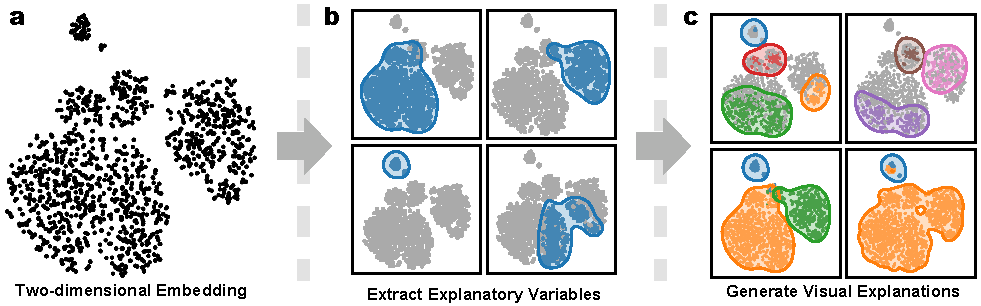
\includegraphics[width=\linewidth]{teaser.pdf}
  \caption{Given an arbitrary two-dimensional embedding (a), VERA identifies spatially-localized explanatory variables (b), and constructs informative explanations, which aim to explain the structure of the underlying embedding (c).}
  \label{fig:teaser}
}

%% Uncomment below to disable the manuscript note
%\renewcommand{\manuscriptnotetxt}{}

%% Copyright space is enabled by default as required by guidelines.
%% It is disabled by the 'review' option or via the following command:
%\nocopyrightspace


%%%%%%%%%%%%%%%%%%%%%%%%%%%%%%%%%%%%%%%%%%%%%%%%%%%%%%%%%%%%%%%%
%%%%%%%%%%%%%%%%%%%%%% LOAD PACKAGES %%%%%%%%%%%%%%%%%%%%%%%%%%%
%%%%%%%%%%%%%%%%%%%%%%%%%%%%%%%%%%%%%%%%%%%%%%%%%%%%%%%%%%%%%%%%

%% Tell graphicx where to find files for figures when calling \includegraphics.
%% Note that due to the \DeclareGraphicsExtensions{} call it is no longer necessary
%% to provide the the path and extension of a graphics file:
%% 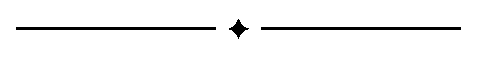
\includegraphics{diamondrule} is completely sufficient.
\graphicspath{{figs/}{figures/}{pictures/}{images/}{./}} % where to search for the images

%% Only used in the template examples. You can remove these lines.
\usepackage{tabu}                      % only used for the table example
\usepackage{booktabs}                  % only used for the table example
\usepackage{lipsum}                    % used to generate placeholder text
\usepackage{mwe}                       % used to generate placeholder figures

%% We encourage the use of mathptmx for consistent usage of times font
%% throughout the proceedings. However, if you encounter conflicts
%% with other math-related packages, you may want to disable it.
\usepackage{mathptmx}                  % use matching math font
\usepackage{amssymb}
\usepackage{amsmath}

\begin{document}

%%%%%%%%%%%%%%%%%%%%%%%%%%%%%%%%%%%%%%%%%%%%%%%%%%%%%%%%%%%%%%%%
%%%%%%%%%%%%%%%%%%%%%% START OF THE PAPER %%%%%%%%%%%%%%%%%%%%%%
%%%%%%%%%%%%%%%%%%%%%%%%%%%%%%%%%%%%%%%%%%%%%%%%%%%%%%%%%%%%%%%%

%% The ``\maketitle'' command must be the first command after the
%% ``\begin{document}'' command. It prepares and prints the title block.
%% the only exception to this rule is the \firstsection command
\firstsection{Introduction}

\maketitle

% Why is dimensionality reduction important?
Two-dimensional, point-based visualizations of high-dimensional data are ubiquitous throughout various domains of science, including biology, economics, chemistry, political science, astronomy, and physics~\cite{Liu2017}.
With the advent of big data, analyzing data sets with tens of thousands of features and millions of samples has now become a commonplace occurrence.
A common step during exploratory data analysis is the visualization of these high-dimensional data sets. 
Today, data science practitioners have a plethora of scalable dimensionality reduction methods at their disposal, including principal components analysis (PCA)~\cite{Jolliffe2002}, linear discriminant analysis (LDA)~\cite{Fisher1936}, FreeViz~\cite{Demsar2007}, multidimensional scaling (MDS)~\cite{Kruskal1978}, t-distributed stochastic neighbor embedding (t-SNE)~\cite{Maaten2008}, and uniform manifold approximation and projection (UMAP)~\cite{McInnes2018}.
These can be used to visually uncover underlying structure, such as clusters, transitions, or outliers, and to support exploratory data analysis and hypothesis generation.

% Why is the interpretation of visualizations hard?
After performing dimensionality reduction, analysts typically next want to inspect the resulting visualization and relate the emergent clusters of data points back to the original input feature space~\cite{}.
Linear methods, such as PCA, LDA, and FreeViz, have intuitive explanations of their inferred dimensions, and their axes can easily be related to the original input features by inspecting the projection loadings. However, these approaches are limited in the types of high-dimensional structures they can uncover.
In contrast, non-linear dimensionality reduction approaches, such as MDS, t-SNE, and UMAP, are able to reveal complex structures and patterns. However, relating the embedding dimensions to the original features becomes very challenging.
Understanding the visual structures revealed by non-linear embeddings can be highly beneficial in practical applications, as it can accelerate hypothesis generation and aid in quickly identifying data collection errors~\cite{}.
Additionally, with the development of ever more scalable dimensionality reduction techniques~\cite{McInnes2018,Linderman2019,Lambert2022}, analysts routinely generates multiple embeddings during exploratory data analysis using different parameter settings and algorithms, each potentially revealing distinct aspects of the underlying data manifold~\cite{}.
Subsequently, each resulting visualization must be manually inspected, which can be time consuming and laborious, indicating the need for automated approaches for explaining resulting embeddings to end users.

% Currently, most aproaches are interactive. Why is this not okay?
% - Maybe mention this is only for tabular data
Inspecting and interpreting a two-dimensional embedding typically involves loading data into an interactive tool of choice, using manual selection to inspect visual structures, relating these back to the original input features, and annotating the resulting data map~\cite{}.
Although interactive tools are undoubtedly very powerful and enable users to inspect every aspect of the visualization at a very granular level, when performing exploratory data analysis, users typically first want a rough overview of the characteristics of the embedding space, particularly when generating large numbers of embeddings generated by different parameter settings and dimensionality reduciton algorithms.
The process of annotating the resulting data map is fairly straightforward. Users typically select a group of points, inspect their distribution of the orignal features and compare it to the distribution of the remaining data points. This process must then be repeated for all different input features and for all visual structures in the embedding. %TODO: This sentence is a bit repetitive
Many interactive tools aim to facilitate this process as best as possible using automatic clustering, feature ranking, or automated identification of discriminative features. However, ultimately, these tools still require some degree of user interaction, placing the brunt of the cognitive load onto the end user.
Due to the repetitive nature of this process, comprehensive interactive tools are like overkill. They place a lot of cognitive load on the end user and require them to spend a long time manually sifting through visualizations for what is otherwise a fairly straightforward task.
Therefore, when faced with larger numbers of embeddings requiring interpretation, using automatically generated, static methods may be prefered. Static tools can be easily incorporated into automated pipelines, simply providing the embedding explanation as a result of the pipeline.
Although less powerful and thorough than interactive methods, static tools can provide a quick, big-picture overview of the embedding space. Then, once the analyst has identified an embedding of interest, they would then perform a thorough investigation using their interactive tool of choice, drilling into the different features of the embedding space.

%Although several static embedding explanation approaches have been proposed, these are often limited to a single explanation~\cite{DaSilva2015,VanDriel2020,Tian2021} or require the user to sift through large numbers of explanations~\cite{Faust2019,Plumb2020}.

%Furthermore, many of these tools and their implementations are limited to only one~\cite{Chatzimparmpas2020} or a handful of algorithms~\cite{}.

% What did we do? What problems did we solve? Why is this new?
The address the problems highlighted above, we propose \textit{Visual Explanations via Region Annotation (VERA)}, a static tool for generating visual explanations of a given embedding. VERA requires no user input and automatically identifies the most spatially interesting high-dimensional features in a given two-dimensional embedding. While many explanation approaches have been developed for aiding in the interpretation of two-dimensional embeddings, VERA is the first to specifically algorithmically generate informative, static visual explanations, requiring no human interaction, while retaining the same informative as interactive approaches.

\section{Related Work}
\label{sec:related_work}

Alongside the development of numerous dimensionality approaches for visualization~\cite{Kruskal1978,Maaten2008,McInnes2018}, various visualization tools have been developed to aid in establishing trust and understanding in the resulting embeddings.

One prominent avenue of research has focused on identifying distortions in embeddings, which are inevitably introduced during any dimensionality reduction process. Visual approaches range from visualizing local measures of stress~\cite{Schreck2010,Seifert2010} and neighborhood preservation metrics~\cite{Aupetit2007,LespinatsAupetit2011,Martins2014}, to interactive tools aimed at identifying and correcting distortions~\cite{Heulot2013,Stahnke2016}.
Nonato and Aupetit~\cite{NonatoAupetit2019} provide an excellent overview of embedding distortions and their associated methods.
These methods primarily aim to assess the trustworthness and reliability of the spatial relationships between data samples in the embedding. Our work, on the other hand, aims not to highlight mapping distortions, but to aid users in the interpretation of the resulting embedding space and explain the properties of the emergent visual sturctures.

The idea of helping users in the interpretation of embeddings is not new, and several such approaches and tools have been developed over the years.
Some methods at explain embeddings globally, typically by relating the embedding dimensions to the original, high-dimensional features~\cite{Broeksema2013,Coimbra2016}.
While these approaches work well for linear projections, many modern dimensionality reduction techniques rely on highly non-linear transformations of the original feature space.
Other approaches, instead, focus on explaining local, visual patterns, such as clusters, transitions, and outliers in the embedding space.
All of these methods typically imbue the resulting two-dimensional scatter plot with additional information, aimed at describing the visible structure~\cite{Joia2015,ChengMueller2016,Tian2021}, or provide an interactive interface through which users can navigate and explore the embedding space~\cite{Kandogan2012,Stahnke2016,Bibal2021}.

% Descriptive
Of these local approaches, several aim to identfy characteristic features for visual clusters or regions in the embedding space.
Joia \etal~\cite{Joia2015} develop an SVD-based approach to identify characteristic features in visual clusters.
Da Silva \etal~\cite{DaSilva2015} and subsequent extensions by Van Driel \etal~\cite{VanDriel2020} and Tian \etal~\cite{Tian2021} identify low-variance features in particular regions of the embedding.
Pagliosa \etal~\cite{Pagliosa2016} develop a similar, interactive, variance-based approach, applied more locally via clustering or user selection.
Some other approaches are based on jointly embedding samples and features into the same embedding space.
Broeksema \etal~\cite{Broeksema2013} use multiple correspondence analysis to embed both samples and features into a single embedding space and use Voronoi tessellations to define regions of characteristic feature values in the embedding space.
Cheng and Mueller~\cite{ChengMueller2016} develop a similar, MDS-based approach, in which features are positioned near samples with high values of that particular feature. In their approach, regions are defined using kernel density estimates.

% Contrastive
% TODO can be written better
While identifying characteristic features for particular regions can be insightful and can help in identifying \textit{what} a particular region corresponds to, humans generally tend to prefer contrastive explanations describing the differences between regions~\cite{Miller2019}.
Several approaches have been developed to provide contrastive explanations, highlighting the differences between visual clusters in the embedding space.
Kandogan~\cite{Kandogan2012} uses a combination of custom metrics to identify features distinguishing between clusters in the embedding.
Fujiwara \etal~\cite{Fujiwara2020} identify distinguishing features using contrastive PCA.
Marcilio \etal~\cite{Marcilio2021} use t-tests to identify characteristic features for each particular cluster.
Bibal \etal~\cite{Bibal2021} use decision trees to identify discriminative features between clusters.
Marcilio and Eler~\cite{MarcilioEler2021} use Shapley values to explain clusters in the embedding.

A majority of the mentioned approaches typically provide an interactive interface in which users can explore the embedding space, select and inspect groups of points, and examine their corresponding feature distributions~\cite{Stahnke2016,Chatzimparmpas2020,Eckelt2022}. However, because these approaches typically display a distribution for each feature, they are not scalable when we have a large number of features, as users have to inspect each feature distribution manually.
% Some sentence why interactive interfaces are slow to use

% TODO: Include, but integrate better into the text
%Some efforts have been made to make the mapping more interpretable by enforcing a more interpretable mapping~\cite{Couplet2023}, or finding partial derivatives via perturbations~\cite{Faust2019} or analytically for specific dimensionality reduction algorithms~\cite{Scicluna2023}. This is fine, but requires the modification of all the algorithms, some of which may not be possible. Additionally, this can deteriorate the quality of the resulting embedding. And, adoption will be low since people aready use their own tools.


%For instance, Sohns et al.~\cite{Sohns2022} develop rangesets, a visualization technique to help the user visualize regions in the embedding where particular value ranges of a specific variable occur.


%Summary paragraph, doing light criticizing of existing methods, say what we improve
Nearly all the aforementioned methods require some degree of user interaction. Most often, clusters need to be selected manually selected or validated by setting hyperparameters in the user interface.
While descriptive methods, aiming to characterize different regions of the embedding space, these explanations are typically less satisfying than contrastive explanations.
Tree-based methods typically identify only a handful of features.
Most approaches are not scalable to a large number of features, since they require users to sift through them all.

Unlike nearly all the aforementioned methods, our approach does not rely on identifying clusters, but is automatically determines different regions of the embedding space which may correspond to visual clusters, but can also characterize individual parts of visual clusters.

\section{Methods}

\begin{figure*}[t]
  \centering
  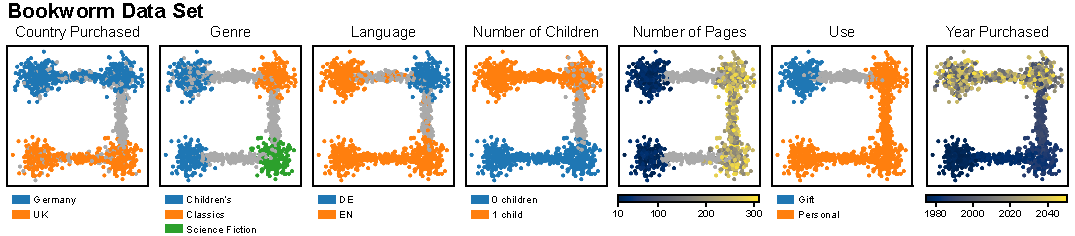
\includegraphics{fig_variable_values.pdf}
  \caption{\label{fig:variable_values}Variable values. We visualize the variable values as they are typically depicted using a scatter plot. Categorical variables are colored with a discrete colormap, while the two numeric variables are colored with a continuous colormap. Missing variables are colored gray.}
\end{figure*}

In this section, we describe \textit{Visual Explanations via Region Annotation (VERA)}, our proposed approach for generating static visual explanations for a given two-dimensional embedding.
Miller~\cite{Miller2019} posits that explanations involve three cognitive processes: explanation generation, selection, and evaluation. In this work, we aim to automate the first and second of these cognitive processes. In the first step, we generate several potential explanations, then rank and select the most salient explanations in the second step to show to the end user. The evaluation step is ultimately left to the end user, as only they can evaluate the usefulness of an explanation for their particular problem.

Before proceeding, we first define the necessary terminology. 
Given an arbitrary dataset $D \in \mathbb{R}^{N \times |F|}$ comprised of a set of high-dimensional features $F$ and its corresponding two-dimensional embedding $Y \in \mathbb{R}^{N \times 2}$, our aim is to visually relate different regions of $Y$ back to the original, high-dimensional features $F$.
We refer to each high-dimensional feature $f \in F$ as a \textit{base variable}.
Base variables can take on a wide range of values, some of which may be characteristic of particular regions of $Y$. For instance, data points in a particular cluster may all share the same category for some categorical feature or contain similar values for some numeric feature.
We package these informative values into \textit{rules}, which typically define some particular categorical value or some numeric interval of values.
A rule $\varphi_i$ is defined as a function $\varphi: Y \rightarrow \left \{ 0, 1
\right \} $, which evaluates to $1$ if the condition is met for a given data sample and $0$ otherwise.
Rules are associated with \textit{regions} via \textit{explanatory variables} $e_i$, which represent pairs of rules $\varphi_i$ and regions $r_i$, $e_i = \left ( r_i, \varphi_i \right )$.
Each region $r_i$ represents a set of points $r_i = \{ y_1, y_2, \cdots, y_N \} \subseteq Y$, contained within the region.
Once we have identified a set of explanatory variables $E = \left \{ e_1, e_2, \cdots, e_K \right \}$, we next want to display these to the user. Simultaneously displaying all $K$ explanatory variables to the user in a single plot would be no good, as it would almost certainly lead to region overlap, illegible labels, and a general information overload.
Instead, we group explanatory variables into collections of explanatory variables to avoid overlap and that follow the principles of contrastive explanation. We refer to each such collection as a \textit{panel} $P \subseteq E$. We refer to each panel as a \textit{visual explanation} and use the two terms interchangeably.
Finally, a single panel will typically convey information about a single base variable or group of correlated base variables or may show a single partitioning of the embedding space.
Therefore, we show the user a user-specified number of panels. We refer to a collection of panels as a \textit{layout} $L = \left \{ P_1, P_2, \cdots, P_L \right \}$.
% TODO: Explanatory variable groups, regions are merged by taking the union of the underlying samples.

We describe the two different types of visual explanations we propose in this work.
\textit{Constrastive explanations} typically consider a single base variable and show where in the embedding space particular values of that variable are enriched.
\textit{Descriptive explanations}, on the other hand, aim to describe what feature values are characteristic for different regions of the embedding space.
Contrastive explanations are useful for answering questions like ``Where do the different values of this feature occur?''
On the other hand, descriptive explanations aid in answering questions like ``What feature values are characteristic for this cluster?''.

We will illustrate the different stages of our approach through a fictional, guiding example.
We construct a synthetic data set in which each point corresponds to a book owned by a fictional lover of the literary arts.
The data set is comprised of seven features: book language, genre, number of pages, purchase year and country, whether or not they had children at the time of purchase, and whether or not the book was purchased for personal use or as a gift.
A two-dimensional embedding of this data set is provided in advance, showing four distinct clusters of books connected by three transitions. The embedding, colored by the seven different feature values, is shown in Fig.~\ref{fig:variable_values}.

Through these books, we can trace the life of this fictional bookworm. The books in the bottom left cluster give us a peek into their childhood; the cluster is filled with children's books, presumably given to them by their parents. Their teenage years are characterized by the bottom right cluster, filled with longer science fiction books. After spending their formative years in the United Kingdom, they packed up their belongings and made Germany their new home, where their literary tastes switched to German literary classics, which remained their favorite books to this day. Soon thereafter, they had their first child, which they also decided to raise with an appreciation for literature. However, to ensure their child be instilled with a sense of British national pride, they stubbornly allowed their child to read only books in English.

In the subsequent sections, we will use VERA to uncover these same conclusions, but in an automated fashion.


\subsection{Region Construction}
\label{sec:region-construction}

Regions serve as the fundamental building block for constructing visual explanations.
Regions represent collections of data points in the embedding sharing a common characteristic.
A region is a collection of one or more polygons in the embedding space, each encompassing a set of data points. Ideally, a region should contain all data points with that characteristic and exclude all other data points. However, in most real-world embeddings, a clean separation between points with some particular feature value and those without rarely exists.

Briefly, our procedure is as follows: for each high-dimensional, base variable, we group samples based on their feature values, determining informative ranges of numeric values or particular categories. We then pair each semantic rule with a spatial region of the embedding space in which the data points satisfy the rule.
We illustrate the region construction process in Fig.~\ref{fig:region_construction}.

\begin{figure*}[t]
  \centering
  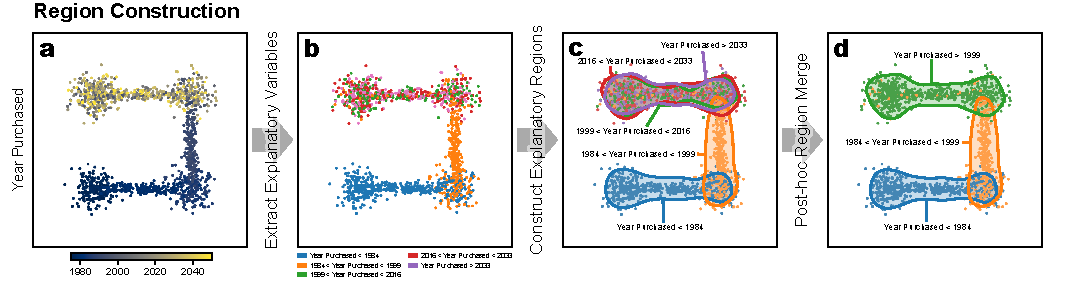
\includegraphics{fig_construct_regions.pdf}
  \caption{\label{fig:region_construction}We illustrate the region construction process for a single variable using a synthetic example. (a) Coloring points by a particular feature value is a common way of inspecting low-dimensional embeddings. However, this inspection can be difficult in the presence of outliers that skew the color scale. (b) We discretize the numeric values into five bins, resulting in five binary indicator variables. Categorical variables do not need to be discretized, and binary indicator variables are obtained via one-hot encoding. Points here are colored according to their discretization bin membership. (c) For each of the discretized bins, we obtain regions in which these values are enriched. (d) After region merging, highly overlapping regions are merged.}
\end{figure*}

\subsubsection{Extracting Explanatory Variables}

An input data set $D$ can contain both categorical and numeric variables. Since we want to explain the embedding in terms of the base variables' values, we must first identify reasonable values or value ranges that correlate with the embedding space. % TODO: A bit strangely written --correlate with the embedding space--
We discretize numeric variables into $k$ binary indicator variables using $k$-Means quantization. By default, we construct five bins corresponding to the typical five-point scale: ``very low'', ``low'', ``medium'', ``high'', and ``very high''. For instance, the numeric variable in Fig.~\ref{fig:region_construction}.a is discretized into five bins, shown in Fig.~\ref{fig:region_construction}.b. Categorical variables are one-hot encoded, resulting in $k$ binary indicator variables, each corresponding to a particular category. Each indicator variable is associated with a rule $\varphi_i$ indicating its discretization interval or category selection.

This procedure expands each base variable into a collection of explanatory indicator variables, each corresponding to a particular range of numeric variables or a specific category of categorical variables. Each explanatory variable is then associated with a \textit{rule}.

\subsubsection{Constructing Explanatory Regions}

To construct regions, we adopt a procedure similar to that of \textit{splatterplots}~\cite{MayorgaGleicher2013}. For each binary indicator variable, we obtain the kernel density estimate (KDE) $D$ using a Gaussian kernel. Next, we extract the contours of the density estimate at a user-specified level, defaulting at $0.25 \cdot \max D$.
In our running example, Fig.~\ref{fig:region_construction}.c shows the five regions constructed from the five bins shown in Fig.~\ref{fig:region_construction}.b.
Note that, in general, the KDE may be multimodal, and we may end up with more than one polygon. This happens when an explanatory variable is enriched in multiple regions of the embedding space.

An important consideration is how to set the kernel bandwidth $\sigma$ of the Gaussian kernel used during the KDE step.
Different embedding algorithms produce embeddings that can span across different scales, e.g., one embedding may span from $-1$ to $1$ along its dimensions, while another may span from $-10$ to $10$.
Additionally, a single scale parameter may not be desirable for data sets containing different numbers of samples. For instance, in a dataset with 50 samples, we are likely interested in groups of 10-20 points, while in a dataset containing 2 million samples, the groups of interest are likely larger.
We here set the scale to equal the median distance of each point's $k$-th nearest neighbor, where we set $k=\sqrt{N}$.

This procedure imbues each explanatory variable $e$ with an associated region $r_i$. Each resulting explanatory variable $e_i$ contains a rule $\varphi_i$ and region $r_i$, thus concluding the explanatory variable construction process.

\subsubsection{Post-hoc Region Merging}
\label{sec:post-hoc-merge}

When discretizing numeric variables, it is unlikely that five bins will result in the optimal discretization.
For instance, in Fig.~\ref{fig:region_construction}.c, the values in the top section of the embedding have been discretized into three bins. The resulting overlapping regions clutter the visualization, making it difficult to read. Spatially, however, these three regions exhibit nearly perfect overlap and could be merged into a single region, more clearly conveying the same information.
It is easy to envision a similar scenario with multiple overlapping categories for categorical variables.
To reduce spatial overlap, we apply a post-hoc merging procedure to the explanatory variables obtained from the previous steps.
At this phase, we only consider merging explanatory variables originating from the same base variable.

When considering regions to be merged with one another, we must first ensure a sufficiently high degree of spatial overlap between the two. We define the \textit{maximum overlap} between two regions $r_i$ and $r_j$ as
\begin{equation}
\text{max\_overlap}(r_i, r_j) = \max \left \{ \frac{|r_i \cap r_j|}{|r_i|}, \frac{|r_j \cap r_i|}{|r_j|} \right \}, \notag
\end{equation}
where $|r|$ denotes the number of points within the region.
The maximum overlap ensures that if a small region is completely contained within a much larger region, the two regions are merged.
To merge two regions, we require that their maximum overlap exceeds a user-specified threshold, in our case defaulting to $0.5$.

Each explanatory variable is comprised of a region $r_i$ containing points $y_i$, and a rule $\varphi_i$. While many of the contained points $y_i$ satisfy this rule by construction, the region may also contain points that do not. We refer to these points as true members and false members, respectively. To quantify the proportion of true members in a region $r$, we define the \textit{purity} of a region $r_i$ as
\begin{equation}
\text{purity}(r) = \frac{1}{|r|} \sum_{y_i \in r} \varphi_i (y_i). \notag
\end{equation}
Merging two low-overlap regions can result in a decrease in purity in the resulting explanatory variable. Low-purity regions are unreliable, as many of the encompassed data points do not actually satisfy the associated rule.
To quantify the effect of a potential merge on purity, we define the purity gain of a potential merge between two regions as
\begin{equation}
\text{purity\_gain}(r_i, r_j) = \max \left \{ \frac{\text{purity}(r_{\text{new}})}{\text{purity}(r_j)} - 1, \frac{\text{purity}(r_{\text{new}})}{\text{purity}(r_j)} - 1 \right \}, \notag
\end{equation}
where $r_{\text{new}}$ denotes the merged region $r_{\text{new}} = r_i \cup r_j$.
To avoid reducing region purity and ensure the reliability of the merged explanatory variables, we require that their maximum purity gain exceeds a user-specified threshold, in our case defaulting to $0.5$.

Alongside spatial and purity constraints, we also impose semantic rule constraints to account for the compatibility between the rules associated with the two explanatory variables to be merged.
For ordinal and numeric variables, we only allow merging consecutive bins. For instance, the rules produced by discretization $\{ x < 5, 5 \leq x < 6, 6 \geq x\}$ for a numeric variable could be merged into $\{x < 6, 6 \geq x\}$, but not into $\{ 5 \leq x < 6, x < 5 \mid x \geq 6\}$.
The same reasoning applies to ordinal categorical variables, merging only adjacent categories. For instance, the ordinal values $\{1, 2, 3, 4\}$ could be merged into $\{\{1, 2, 3\}, \{4\}\}$, but not into $\{\{1, 4\}, \{2, 3\}\}$.
We apply no such restriction to nominal categorical variables. For example, the categorical variable values $\{red, green, blue\}$ could be merged into $\{\{red, blue\}, \{green\}\}$.

If a pair of explanatory variables satisfies all these criteria, the two can be merged into a new explanatory variable, with their rule appropriately updated and regions merged. We implement this approximately by first constructing a graph, placing edges between compatible explanatory variables, identifying the connected components in the graph, and merging the identified groups.

For instance, in our running example in Fig.~\ref{fig:region_construction}, consider the top section of the embedding in Fig.~\ref{fig:region_construction}.c. The three regions have a near-perfect degree of overlap, giving them a maximum overlap close to 1. Since the three regions evenly share the underlying data points, the purity of the individual regions will be near $1/3$. Merging any two of these regions would include roughly $2/3$ of the points, giving a purity gain of $\sim2$. Finally, the three rules are semantically compatible and can be merged into a single, open-ended interval. The final, merged explanatory variable is shown in Fig.~\ref{fig:region_construction}.d.

Features whose values exhibit no spatial correlation with the embedding space are merged into a single explanatory variable. These variables hold no explanatory power and are discarded from subsequent steps.
Additionally, having obtained our final explanatory variables, we can filter them to satisfy some minimum number of members to avoid showing small, spurious regions or a minimum purity to avoid displaying unreliable regions.

The result of our region construction procedure is as follows: for each of the high-dimensional, base variables, we generate one or more explanatory variables, which, together, describe the entire range of the feature's values. To mitigate overfragmentation, we apply a post-hoc merging procedure, which merges spatially overlapping and semantically compatible explanatory variables. The result is that each base variable becomes associated with a varying number of explanatory variables. Base variables associated with a single explanatory variable hold no informative value as their underlying values do not exhibit any spatial localization and are discarded.

\subsection{Contrastive Explanations}
\label{sec:contrastive}

Contrastive explanations show where particular values of a given base variable occur in the region. This is akin to coloring points in a scatter plot based on their feature values, one feature at a time, but with several advantages. Firstly, our procedure filters out features that are not spatially interesting and ranks the remaining features in terms of their information content. This way, the user does not need to sift through the various features to determine the relevant ones. Secondly, by performing discretization, our approach mitigates the problem of outliers skewing color bars.

\subsubsection{Explanation Construction}

The region construction process splits each base variable into a set of explanatory variables, each occupying its own region of the embedding space. While we could directly construct panels of explanatory variables for each base variable, we can further refine the explanatory variables for contrastive explanations.

We devise the \textit{contrastive merge}, which merges spatially overlapping explanatory variables from different base variables into explanatory variable groups. Unlike the post-hoc merging procedure described in Section~\ref{sec:post-hoc-merge}, where we limited merging to explanatory variables from a single base variable, we here consider pairs of explanatory variables between different base variables.
To perform a contrastive merge between two base variables $v_1$ and $v_2$, we require that each explanatory variable $e_i \in v_1$ has a spatially overlapping $e_j \in v_2$. If such a bipartite matching is identified, we merge the explanatory variables, representing the two base variables with a single explanatory variable group.
For instance, the two panels depicting two base variables in Fig.~\ref{fig:contrastive_merge} exhibit perfect overlap and are subsequently merged into a single panel.
This procedure not only reduces the number of panels needed to convey the same amount of information but can also reveal potentially non-linear correlations between high-dimensional features.

\begin{figure}[t]
  \centering
  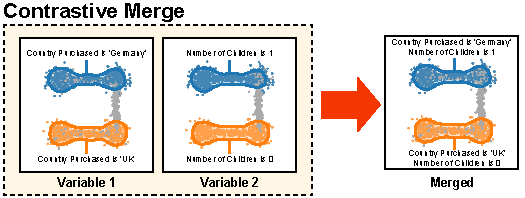
\includegraphics{fig_contrastive_merge.pdf}
  \caption{\label{fig:contrastive_merge}The contrastive merge. If two base variables comprise explanatory variables whose regions have a perfect overlap bipartite matching, we can merge the explanatory variables into explanatory variable groups. This not only reduces the number of panels a user needs to inspect but also highlights correlations between particular variable values.}
\end{figure}


\subsubsection{Explanation Selection}
\label{sec:contrastive-selection}

Generating contrastive explanations is straightforward: We simply generate panels containing all explanatory variables associated with each high-dimensional, base variable.
However, on its own, this provides little benefit to the end user, as they would then have to sift through the potentially large number of panels by hand.
Instead, we develop a ranking procedure that identifies the most informative base variables and orders them by relevance.

To identify the most informative features in a given two-dimensional embedding, we compute the following metrics for each candidate panel:
\begin{itemize}
  \item \textit{region overlap}: features whose values are localized to particular regions of the embedding space are likely to be more interesting than features with a more even distribution of feature values along the embedding. By design, the first kind of features will exhibit lower overlap than non-correlated features. We compute the overlap between two explanatory variables as the Jaccard similarity of their regions. To obtain the total overlap of a panel $P$, we compute the mean overlap between all pairs of explanatory variables $(e_i, e_j) \in P \times P, i \neq j$.
  \item \textit{mean purity}: the purity of each region indicates what proportion of the samples encompassed by the region satisfy the associated rule. High-purity regions should be preferred, as these are much stronger patterns than low-purity regions.
  \item \textit{number of items}: An often cited result from psychology is that humans generally have a limited working memory, being able to hold only a handful of items in their attention at a time. Several bounds on this number of items have been proposed, including seven~\cite{Miller1956}, four~\cite{Cowan2001}, and two~\cite{Gobet2004}. We apply these findings to explanation selection, using an intermediate estimate of 3. Panels containing a large number of explanatory variables place more cognitive load on the user and are less likely to be informative than simpler panels containing only a handful of regions. Therefore, we score each panel based on the number of contained explanatory variables $\left | 3 - |P| \right |$.
\end{itemize}
Then, we compute the rankings of the panels along each score. To obtain a single, final panel ranking, we compute the weighted sum of individual metric rankings and select the panel with the highest overall ranking. We repeat this process for as many panels as the user requests. This process is illustrated in Fig.~\ref{fig:contrastive_generation}.

\begin{figure}[t]
  \centering
  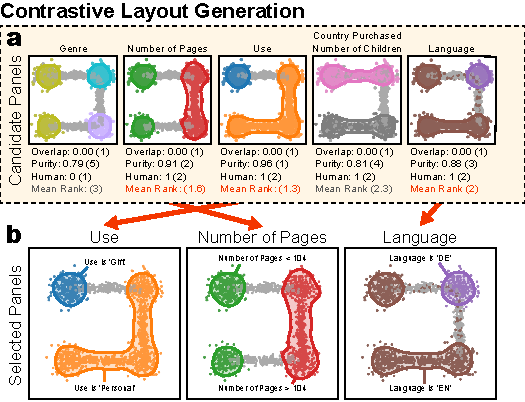
\includegraphics{fig_contrastive_selection.pdf}
  \caption{\label{fig:contrastive_generation}Contrastive layout generation. (a) Generating candidate panels simply involves including all explanatory variables associated with a particular base variable in a separate panel. Each candidate panel is scored and ranked according to three metrics, and a weighted mean rank is computed for each panel. (b) The top $k$ panels with the highest mean rank, indicated in red, are included in the resulting layout.}
\end{figure}


\subsection{Descriptive Explanations}

Descriptive explanations describe regions of the embedding space by determining sets of features and feature values characteristic for that particular region. Unlike contrastive explanations, which generally display a single base variable, these visualizations identify overlapping explanatory variables across different base variables, uncovering potentially interesting relationships between specific variable values.

\subsubsection{Explanation Construction}

\begin{figure}[t!]
  \centering
  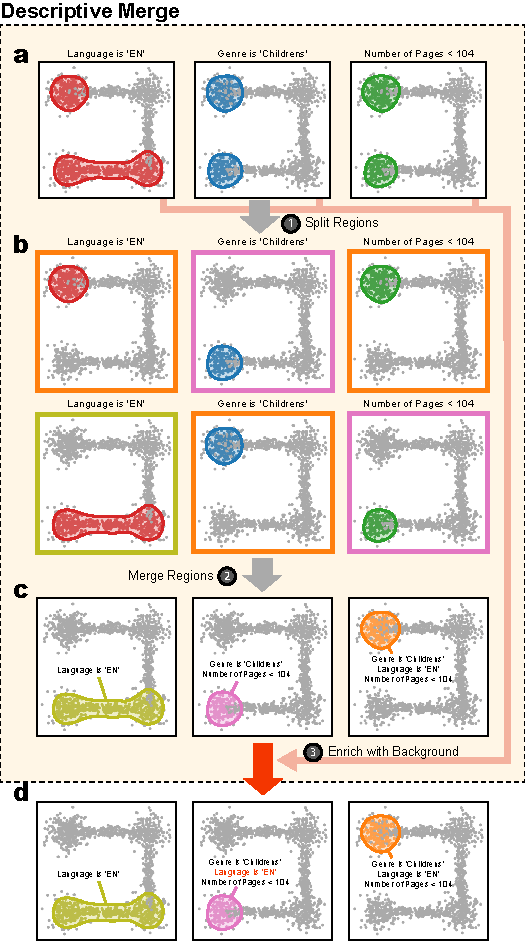
\includegraphics{fig_descriptive_merge.pdf}
  \caption{\label{fig:descriptive_merge}Descriptive merge}
\end{figure}

As in contrastive explanation construction, the regions produced by the procedure outlined in Section~\ref{sec:region-construction} provide a good starting point for generating explanations, but can be further refined to convey descriptive information using the \textit{descriptive merge}.

The descriptive merge procedure follows three basic steps. In the first step, each explanatory variable produced in Section~\ref{sec:region-construction} is split into new explanatory variables based on the number of regions it contains. Oftentimes, particular feature values occupy multiple regions of the space, resulting in multiple enriched regions. If an explanatory variable contains only a single region, it is not split. For instance, the three explanatory variables shown in Fig.~\ref{fig:descriptive_merge}.a are each comprised of two regions, each of which is split into two explanatory variables in Fig.~\ref{fig:descriptive_merge}.b.

In the second step, we collect the separated explanatory variables and identify overlapping regions, which we merge into explanatory variable groups. 
Two explanatory variables can be merged if they reach a sufficiently high degree of spatial overlap. We define the \textit{maximum overlap} between two regions $r_i$ and $r_j$ as
\begin{equation}
\text{min\_overlap}(r_i, r_j) = \min \left \{ \frac{|r_i \cap r_j|}{|r_i|}, \frac{|r_j \cap r_i|}{|r_j|} \right \}. \notag
\end{equation}

This approach is reminiscent of the post-hoc region merge procedure described in Section~\ref{sec:post-hoc-merge}, where we required the maximum overlap to exceed a particular threshold. There, the maximum overlap metric ensured that smaller regions contained within larger regions get absorbed into the larger region. Here, adopting this approach would mislead the user. Consider two explanatory variables $e_i$ and $e_j$ associated with rules $\varphi_i, \varphi_j$ and regions $r_i, r_j$ respectively. If $r_j$ corresponds to a small region, entirely contained within the much larger region $r_i$, the new, merged explanatory variable $e_{\text{new}}$ would indicate that the points within the new region satisfy both rules $\varphi_i$ and $\varphi_j$. Because regions are merged by taking the union of $r_i$ and $r_j$, the majority of points in $e_{\text{new}}$ would not satisfy rule $\varphi_j$ and would be misleading to the user. Regions like this would also be filtered out if purity-based filtering is applied. By using the minimum overlap instead of the maximum overlap, we ensure that only well-overlapping regions are merged.

The merged regions produced in the previous step contain rules originating from regions with nearly perfect overlap. However, these new regions can be subsets of larger regions with their own associated rules. Provided the regions have sufficiently high maximum overlap, we add rules from larger regions to the smaller, newly formed regions. Importantly, we do not merge the regions; we only add rules to the smaller regions.
For example, in Fig.~\ref{fig:descriptive_merge}.c, the middle pink region represents shorter children's books, obtained by merging the perfectly overlapping regions in Fig.~\ref{fig:descriptive_merge}.b. However, all these books are also contained within the yellow region in the left panel, which corresponds to English books. Therefore, in Fig.~\ref{fig:descriptive_merge}.d, we enrich the pink explanatory variable with the rule from the encompassing yellow region, indicating these are all shorter English children's books. We refer to this process as \textit{background enrichment}.
While this step, in theory, provides overlapping functionality as the merging procedure, in practice, one would then have to account for detecting nearly duplicate explanatory variable groups.


\subsubsection{Explanation Selection}

\begin{figure*}[t!]
  \centering
  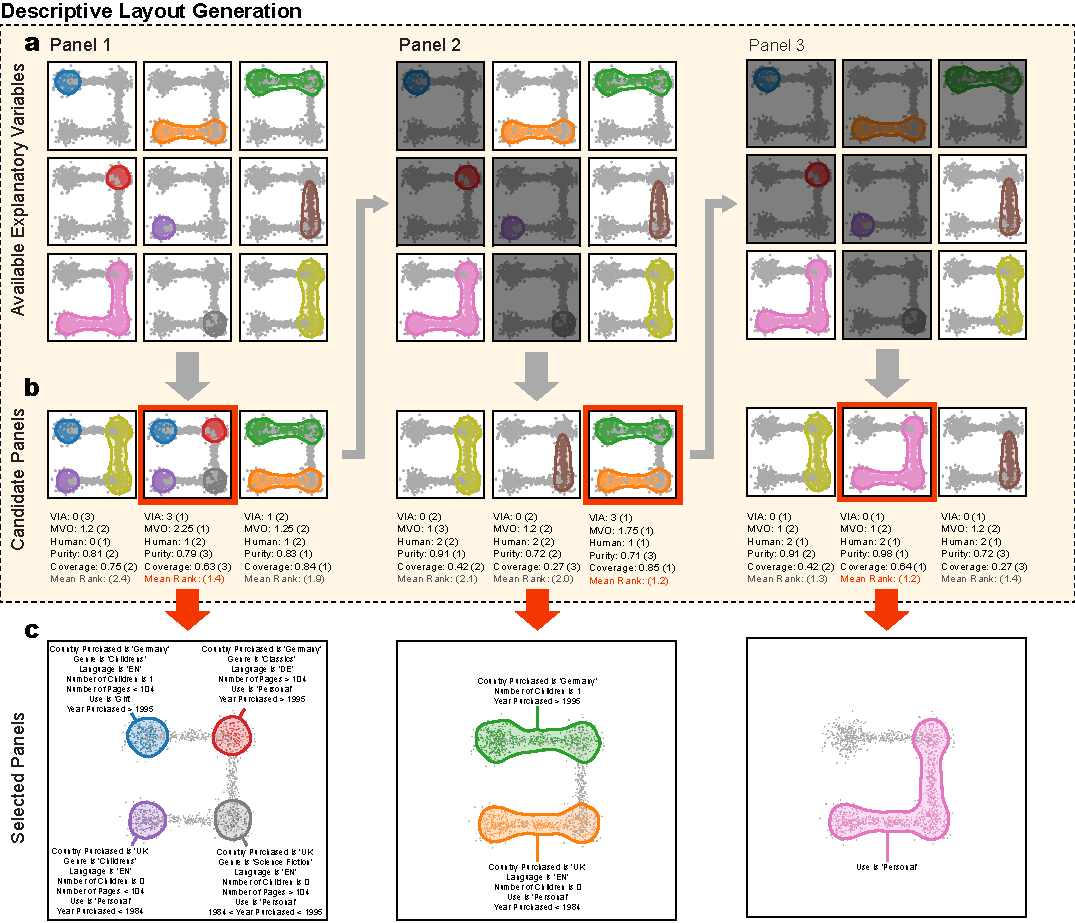
\includegraphics{fig_descriptive_selection.pdf}
  \caption{\label{fig:descriptive_generation}The descriptive layout generation follows an iterative approach. Given a set of available explanatory variables in (a), we identify non-overlapping combinations of these to be used as candidate panels. We show three such candidate panels in (b). Then, each panel is scored along the five different metrics, which are subsequently ranked and averaged. The panel with the highest mean rank, indicated in red, is added to the resulting layout, shown in (c). Finally, we remove the explanatory variables in the selected panel from the set of available explanatory variables. We then repeat the procedure until we generate a specified number of panels or until we run out of explanatory variables.}
\end{figure*}

Descriptive explanations are generated and selected in an iterative fashion.
Given an initial set of available explanatory variables $S_0$ produced by the descriptive merge procedure outlined above, we first identify all potential combinations of explanatory variables such that the overlap between regions does not exceed some prespecified threshold. We cast this as an independent set problem, where each node in the graph corresponds to a particular explanatory variable, and edges are placed between them where the overlap between their corresponding regions exceeds the prespecified threshold. The independent sets correspond to collections of non-spatially overlapping regions, which are then considered candidate panels.

A key consideration when generating descriptive explanations is how to enforce the principles of contrastive explanation.
In contrastive explanations, the panels show regions of different feature values for single base variables and are contrastive by nature.
Here, however, each panel can contain explanatory variables comprised of wildly different base variables. In this case, a user may not be able to compare regions with one another inside a single panel, as the different regions may correspond to different high-dimensional features.

To enforce a level of contrastivity within descriptive explanations, we score each panel according to its \textit{mean variable occurrence} (MVO). The MVO counts the occurrence of each included base variable in the explanatory variables and reports the mean value. If a base variable appears in all explanatory variables in a given panel, we assign a special  \textit{variable in all} (VIA) score of 1 and 0 otherwise.

Additionally, we score each panel according to its \textit{sample coverage}, i.e., what proportion of all data points are contained within any given region in the panel. We also include the \textit{mean purity} and \textit{number of items} metrics from Section~\ref{sec:contrastive-selection}, preferring panels with high-purity regions and panels with a reasonable number of explanatory variables.

In order to select the best panel, we apply the same weighted rank-based approach as in Section~\ref{sec:contrastive-selection} to the five metrics described above.
We insert the most highly-ranked panel $P_{\text{max}}$ into the resulting layout, and the explanatory variables $e_i \in P_{\text{max}}$ are removed from the set of available explanatory variables $S_{t + 1} = S_{t} \setminus P_{\text{max}}$. We repeat the procedure until we generate the requested number of panels or until we run out of available explanatory variables $S$. The procedure is illustrated in Fig.~\ref{fig:descriptive_generation}.


\section{User Scenario}

Here, we present a typical user scenario demonstrating the usage of the generated VERA visual explanations.
As our guiding example, we use the IBM Employee Attrition data set~\cite{IbmEmployeeAttrition}. The data set describes 1,470 fictional employees characterized by 33 features. We obtain a two-dimensional embedding using the t-SNE algorithm using the \textsf{openTSNE} library~\cite{Policar2019}.

\begin{figure*}[t]
  \centering
  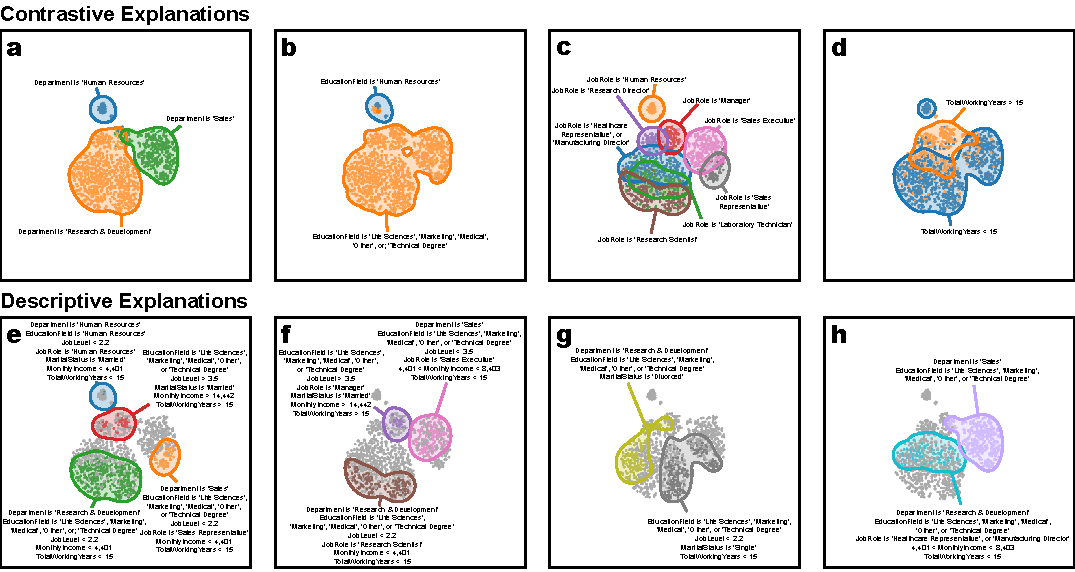
\includegraphics{case_study-attrition.pdf}
  \caption{\label{fig:attrition}VERA explanations of the IBM Employee Attrition data set. Panels (a-d) show four contrastive explanations corresponding to the features that are spatially most correlated with this particular embedding. The descriptive explanations shown in panels (e-h) characterize different regions of the embedding space.}
\end{figure*}

Fig.~\ref{fig:attrition} shows the resulting VERA explanations.
The four contrastive panels in Figs.~\ref{fig:attrition}.a-d show the four most spatially localized features. These indicate that the most salient features separating the clusters in the embedding correspond to the employees' department, education, job role, and total working years. Figs.~\ref{fig:attrition}.a-b show that the primary discriminating features between clusters are the employee department and education field. Fig.~\ref{fig:attrition}.c shows the different job roles, while Fig.~\ref{fig:attrition}.d separates more junior from senior employees.

The four descriptive explanations depicted in Figs.~\ref{fig:attrition}.e-h characterize the different regions of the embedding space. The blue cluster in Fig.~\ref{fig:attrition}.e describes the characteristics of the human resources department, indicating more junior, married individuals with a lower salary. The red cluster identifies more senior, married, and higher-salary individuals. Cross-referencing this panel with Fig.~\ref{fig:attrition}.c, we can see that the majority of these employees are in either managerial or research director roles. We can similarly inspect the other regions to gain further insight into the employees' landscape.

Notice that many of the identified regions do not correspond to particular clusters but characterize particular parts of clusters. For instance, the gray region in Figs.~\ref{fig:attrition}.g corresponds to employees who are single, have been working for fewer than 15 years, and have a low job level. We may guess that these correspond to younger, more junior employees. On the other hand, the employees in the yellow cluster are primarily divorced. We are provided with no information about their job level or total working years. Therefore, we do not assume any particular values about these employees.

This example demonstrates


\section{User Evaluation}
\label{sec:user-study}

To assess the effectiveness of our approach, we performed a comparative user study comparing the speed and accuracy with which users could reason about low-dimensional embeddings with both a traditional interactive data-exploration tool and our newly proposed VERA explanations. If the explanations generated by VERA provide similar informative value as a full-fledged interactive tool but faster, this would indicate a positive result.

\subsection{Study Design}

We opt for the Orange data mining toolkit~\cite{Demsar2013} as our interactive tool of choice due to its ease of use and focus on visual data exploration. In Orange, users use widgets to construct potentially complex data-analysis workflows. Orange includes many standard visualization tools for interrogating two-dimensional non-linear embeddings, including scatter and box plots. A typical workflow in Orange might involve visualizing an embedding in a scatter plot, manually selecting groups of points, and comparing their feature distributions to the remaining data points in a box plot.

We prepare two sets of three data sets each, with varying complexity.
The first data set group $D_1$ comprises the Iris, Employee Attrition, and Raisin data sets. The second data set group $D_2$ includes the Penguins, Titanic, and Wine Quality data sets. The data sets are paired between the two groups to ensure comparable levels of equal complexity. For each data set, participants were asked to answer a series of typical questions during the exploration of two-dimensional embeddings, for instance, ``What makes this cluster different from the remaining clusters?'', ``What characterizes the samples in this cluster?'', and ``Do you notice any trend along this region?''.

We recruited roughly 100 bachelor's students enrolled in the Introduction to Machine Learning course at the Faculty of Computer and Information Science at the University of Ljubljana.
Prior to the study, the participants had some familiarity with Orange and were unfamiliar with VERA explanations. Before conducting the study, we provided a short tutorial on both Orange and VERA explanations.
We randomly assigned participants to one of two user groups. The first group $G_1$ first used Orange to go through data sets $D_1$, then used VERA explanations for data sets in $D_2$. Conversely, the second group $G_2$ first went through the data sets in $D_1$ using VERA, then through the data sets in $D_2$ using Orange.

During the study, we timed how long it took each participant to answer the questions for each data set. We also assessed whether the answer the user provided was roughly correct. Upon completion, we asked participants to answer a final questionnaire in which they could provide feedback related to the two tools.

\subsection{Results}

The results of our study show that participants using VERA explanations performed equally well as participants using Orange but in a significantly shorter amount of time.
The difference in user performance was not statistically significant, with 91\% of participants answering correctly using Orange and 93\% when using VERA (t-test $p=0.084$).
On the other hand, participants from both user groups answered the questions substantially faster when using VERA explanations. On average, participants using Orange required $29$ minutes to complete questions relating to $D_1$ and $23$ minutes to complete questions relating to $D_2$. Conversely, participants using VERA explanations required $21$ and $15$ minutes for each data set group, representing a roughly 33\% increase in speed ($p<0.005$).
These results confirm that participants from both groups were able to answer the questions with roughly the same degree of accuracy but at a faster rate when using VERA explanations.

Interestingly, participants often answered questions by referencing more features when using VERA explanations. On average, participants mentioned $2.0$ high-dimensional features in their answers when generating explanations using Orange, while this number rose to $2.2$ when using VERA explanations ($p=0.04$). This discrepancy could be due to several factors. For instance, when investigating two-dimensional embeddings with an interactive tool, users must typically scroll through the many different features to investigate their correspondence to the embedding space. Participants often stopped their investigation after identifying one or two informative features, potentially missing other equally informative features. VERA explanations, on the other hand, offer all relevant explanations at the same time. While these explanations are limited in the number of features they show, the explanation ranking mechanisms in VERA ensure that users are shown the most salient features first. Therefore, the user simply \textit{sees} all the features and cannot miss them by chance.

In the final feedback questionnaire, we asked participants to document their experience using both tools. Consistent with the quantitative results, most participants (91\%) reported that they were more quickly able to answer the questions using VERA explanations. The majority of participants (77\%) also confirmed that the provided static explanations were equally informative as Orange.
Surprisingly, when asked which tools participants trusted more, 50\% of participants reported trusting both tools equally, 20\% reported trusting VERA explanations more, and 30\% reported trusting Orange more. 
We expected that users would tend to trust full-fledged, interactive toolkits, like Orange, more than static visual explanations, as these tools provide users with multiple methods to verify their findings and allow them to drill into particular parts of the visualization at their discretion. VERA explanations, on the other hand, are static and offer no such facilities, and the user is forced to simply trust the image.

Finally, we asked participants which types of VERA explanations they found more informative and asked them to rate each explanation type based on its usefulness on a typical five-point Likert scale. Consistent with the findings from Miller~\cite{Miller2019}, most participants (75\%) selected contrastive explanations as the most informative, while 15\% found both explanation types equally informative, and 10\% found descriptive explanations more informative.
Contrastive explanations were given a higher overall rating of $4.4$, while descriptive explanations were given a lower overall rating of $3.2$.
We note that this result does not imply that descriptive explanations are not useful but instead highlights the need to use both contrastive and descriptive explanations in tandem.

\section{Limitations and Future Work}

%- scalability
%- better explanations using large language models
%- other data modalities
%- increasing screen-size may reveal more details, multiple scales of resolutions
%- interactive system
%- limitation of user study is that we had semi-small tabular data sets where the features
%- while the idea of contrastive explanations, where we highlight regions of different feature values is not new, for instance, Sohns \etal~\cite{Sohns2021} proposed a similar idea with using polygonal hulls, their approach requires the user to manually specify discretization bins. Additionally, in their approach, the user has to click through the different features, while our approach automatically ranks them in order of interestingness.
%

While we have demonstrated that the visual explanations generated by VERA are useful, the proposed approach still has several limitations that open avenues for future research.

In the present study, we have only considered tabular data in which each feature conveys some human-readable, semantic meaning. Nowadays, analysts routinely deal with data sets of various modalities, for which our approach could also be practical.
For instance, in compositional data sets, such as text corpora and gene-expression data sets, descriptive explanations could be used to identify characteristic groups of words or highly expressed genes for different regions of the embedding space. These may then be used to identify topics or cell types in two-dimensional embeddings.
Applying our proposed approach to other data modalities, such as image, sound, video, and graph data, where semantically meaningful features are scarce, is not straightforward. For these data modalities, more specialized approaches are likely necessary to address the needs of each particular modality.

A second limitation of our approach is that of scaling in the number of features.
The examples highlighted above and the data sets used in the user study involve data sets containing at most 33 features. In its current form, our approach may not perform the best when adding more features.
For instance, contrastive explanations typically show the top $k$ most informative features. As we increase the number of features, more panels are likely to be needed to get a complete picture of all spatially localized features.
Descriptive explanations, on the other hand, suffer from a different limitation. Each descriptive panel typically contains several explanatory variable groups, each displaying their associated rules. As we increase the number of total features, the number of rule descriptors will also increase, leading to information-dense and, eventually, incomprehensible labels.
However, with the recent advances in natural language processing~\cite{}, we could employ large language models (LLMs) to summarize potentially long lists of feature descriptors and show the auto-generated short summaries in place of the long feature descriptors. For text data, LLMs could likewise be employed to generate topic descriptions. Where available, ontologies could be used to perform ontology enrichment analysis to identify more semantically meaningful labels. For instance, in gene-expression data, we might replace long lists of genes with enriched Gene Ontology terms~\cite{GeneOntology2004}, or, in drug prescription data, we might replace lists of drugs with enriched Anatomical Therapeutic Chemical codes~\cite{Policar2023}. These may then also be summarized by an LLM into a shorter, more human-readable label.
The recent advances in LLM research open exciting new avenues of research for the automatic generation of explanations, which benefit not only visual explanations but the entire field of explainable artificial intelligence as a whole.

A final consideration is that of interactivity. While the development of VERA was motivated primarily by the need for fully automated tools to generate static, visual explanations of two-dimensional embeddings, one can easily envision an interactive system in which visual explanations are integrated into a comprehensive, interactive platform.
Interactive systems are very powerful and allow the user to explore the embedding in more detail, enabling them to focus on subsets of the embedding space and drill into the specific visual structures.
Similarly to splatterplots~\cite{MayorgaGleicher2013}, such an interactive system may also consider the available screen space and adjust the levels of shown detail accordingly.
Such a user interface could seamlessly be integrated into existing visual analytics tools such as Orange~\cite{Demsar2013}, complementing its existing tools for interactive data exploration.

% transitions?

\section{Conclusion}

In today's abundance of big, heterogeneous, high-dimensional data sets, unsupervised dimensionality reduction approaches have become vital in exploratory data analysis. These methods help analysts make sense of the vast amounts of data, allowing analysts to visually uncover potentially interesting structures in the two-dimensional map and drive hypothesis generation. Recent algorithmic developments have enabled these methods to scale to massive data sets, and it has become commonplace to generate multiple such embeddings using different algorithms and parameter settings, as each can reveal a different facet of the underlying data manifold. Inspecting each of these embeddings, however, is cumbersome and time-consuming. Typically, analysts interrogate each embedding in an interactive tool, identifying points of interest, investigating their underlying feature distributions, and labeling groups of points with semantic labels. In this manuscript, we aim to automate this somewhat repetitive task.

We here present \textit{Visual Explanations via Region Annotation (VERA)}, a fully automatic approach for generating static visual explanations of arbitrary two-dimensional embeddings. VERA aims to relate different regions of the embedding space to the original high-dimensional features. Importantly, VERA requires no manual human intervention and can easily be incorporated into existing dimensionality reduction pipelines, producing visual explanations as a byproduct of the analysis.
VERA produces two complementary types of explanations.
Contrastive explanations identify the most salient features and show where, in the embedding, particular values of these features occur.
On the other hand, descriptive features aim to describe particular regions of the space in terms of particular high-dimensional feature values.
Following insights from social sciences, we take special care to ensure our explanations follow the principles of contrastivity, ensuring the resulting explanations are as informative and satisfying as possible.
We validate the utility of our approach using a comparative user study, which shows that our visual explanations are as informative as fully-fledged, interactive tools for answering common embedding interpretation tasks. Importantly, however, due to the static nature of our explanations, users are able to gain insight into their embeddings in a significantly shorter amount of time.

Overall, our work contributes to the growing field of interpretable machine learning and offers a new perspective on explaining non-linear embeddings in terms of their original features.

\section{Code Availability and Reproducibility}

Our open-source, Python implentation of VERA is freely-available at \url{https://github.com/pavlin-policar/vera} and is licensed under the BSD-3 license. The materials used to prepare this manuscript are available at \url{https://github.com/pavlin-policar/vera-paper}.

\section{Acknowledgments}
This work was supported by the Slovenian Research Agency grant P2-0209.

\bibliographystyle{abbrv-doi-hyperref}
\bibliography{references}

\end{document}

